\chapter{Trabajos Relacionados}

%Cada capítulo deberá contener una breve introducción que describe en forma rápida el contenido del mismo. En este capítulo va el marco teórico y el estado del arte. (pueden hacer dos capítulos: uno marco teórico y otro de estado del arte)


\section{Marco Teórico}

\ac{PCG-G} centrada en la generación narrativa puede describirse como un área enfocada en la producción de contenido argumental para el marco narrativo de un videojuego. Los enfoques tradicionalmente identificados son: Sistemas basados en Simulación y Sistemas Deliberativos \cite{garbe2019storyassembler}.

Los Sistemas basados en Simulación tienen por característica principal implementar una serie de reglas que rigen al mundo y a los personajes. Estas reglas actúan como una serie de condicionales que reflejan la intención principal de la historia y son en gran medida establecidas por el propio guionista de la historia. Estas restricciones en conjunto con todas las posibles acciones a realizar sirven de base para una generación sistemática de argumentos narrativos secundarios. Debido a esto, este enfoque suele ser considerado levemente caótico.

Por otro lado, los Sistemas Deliberativos comparten las mismas bases que el enfoque previo, más sin embargo, se diferencian por establecer situaciones a ser resueltas. Este plantemiento permite definir estados deseados a los cuales el sistema debe llegar con prioridad. Un sistema basado en este enfoque es \textit{StoryAssembler} \cite{garbe2019storyassembler}, el cual utiliza una librería de contenidos en donde se especifican las limitantes que posee cada fragmento y que posteriormente son presentadas al jugador a través de una narrativa basada en elecciones. 

Con las definiciones previas es posible definir el desenvolvimiento de un \textit{quest}. Los \textit{quests} son por lo general tareas encargadas por los personajes \ac{NPC} de un juego. Consisten en un grupo de acciones que deben realizarse en un orden en específico para poder alcanzar un objetivo (la mayoría de veces una recompensa) \cite{breault2018let}. Los \textit{quests} representan una parte del contenido narrativo por lo que su desenvolvimiento debe ir acorde con el estado del mundo y la actitud de los \ac{NPC}. Bajo este marco, un \textit{quest} derivado de la aplicación de un sistema \ac{PCG-G} implica el uso de un Agente Inteligente de Planeamiento. Debido a la similitud estructural entre los resultados de estos agentes y el contenido de un \textit{quest}, es posible implementar sistemas como \cite{doran2011prototype} \cite{riedl2011game} \cite{yu2012sequential} en donde historias creadas por humanos son modificadas por IAs de planeamiento siguiendo una serie estados en donde se definen el inicio y el orden de eventos. También es importante destacar que en el orden se debe considerar con prioridad un correcto progreso Lógico-Causal que refleje que los eventos ocurridos a lo largo de la historia obedecen a reglas que favorecen la \textbf{credibilidad del personaje}(percepción por parte del jugador en  donde un personaje actúa de manera coherente).

Enfocado el tema de \textit{quests} podemos clasificarlos en tres categorías segun \cite{cheong2016planning}

\begin{itemize}
\item[•] \textit{Place Oriented Quests} son aquellos en donde el jugador debe de moverse por el mundo hacia un lugar especificado y con ciertas pruebas a lo largo del camino.
\item[•] \textit{Time Oriented Quests} son aquellos considerados como pruebas de resistencia en donde el jugador debe sobrevivir durante un determinado periodo de tiempo.
\item[•] \textit{Objective Oriented Quests} son aquellos caracterizados por la necesidad de cumplir un objetivo (Conseguir un objeto, traer un aliado, eliminar un enemigo, etc.)
\end{itemize}

Todas estas categorías pueden mezclarse de manera tal que mientras se respete el marco narrativo, hagan más atractiva la experiencia del jugador.

Cuando los \textit{quests} queden sujetos a definición por un Agente Inteligente de Planeamiento (A partir de ahora un Planificador), se debe considerar que tanto para un Sistema basado en Simulación como un Sistema Deliberativo, dicho Planificador deberá poseer un conocimiento total sobre todos los posibles eventos que pueden llegar a suceder. Esto incluye la definición de el Estado Inicial (descripción inicial del mundo) así como la definición de el Estado Objetivo (hacia donde debe llegar el Planificador). El objetivo de Planificador es encontrar una solución entre ambos estados, siendo la solución al problema de planeamiento un \textit{Plan} que contenga toda una secuencia de acciones. Cuando el Planificador es capaz de encontrar una solución entre el estado inicial y el estado objetivo, el resultado se conoce como \textit{Sound Plan} \cite{cheong2016planning}.

Por otra parte, el conjunto de eventos que maneja un Planificador se almacena como una librería de sucesos que toman el nombre de \textit{Operadores de Planeamiento} en donde cada operador está compuesto por un conjunto de \textit{Precondiciones} y un conjunto de \textit{Efectos}. Las Precondiciones representan las condiciones que deben alcanzarse para ejecutar el Operador mientras que los Efectos con condiciones que se vieron actualizadas tras el uso del Operador. Las soluciones obtenidas con la aplicación de estos operadores pueden representarse de dos maneras: 

\begin{itemize}

\item \textbf{Soluciones en el Espacio de Estados: } Es una representación en donde las soluciones son estructuradas en un árbol compuesto por nodos y arcos. En esta representación cada nodo es un estado y cada arco es la transición de un estado a otro tras la aplicación de un Operador. Si partimos del nodo raíz, este representará el Estado Inicial del mundo mientras que si nos dirigimos a este, este pasará a ser el Estado Objetivo

\item \textbf{Soluciones en el Espacio de Planes: }  Similar a la representación previa, en esta representación el árbol se vale solo de los nodos para figurar cada solución.  El nodo raíz almacena el problema de planeamiento, el Estado Inicial y el Estado Objetivo. Si no existe una solución directa entre ambos estados, el árbol proyecta un nodo hijo de la raíz en donde se añade un paso más para alcanzar la solución. Si este nodo hijo no alcanza la solución, este proyecta un nuevo nodo hasta que la solución se satisfaga. En esta representación, las hojas del árbol son soluciones completas o soluciones vacías.

\begin{figure}[tph!]
\centerline{
\includegraphics[totalheight=7cm]{3}}
    \caption{Grafo con Soluciones en el Espacio de Planes. \cite{cheong2016planning}}
    \label{fig:ptest1}
\end{figure}


\end{itemize}

\subsection{Planning Story}

La representación de una historia derivada del uso de un Planificador puede definirse como una Tupla: $<S, O, C>$ en donde :

\begin{itemize}
\item S es un conjunto de eventos procedente de la librería de Operadores.
\item O representa el orden temporal entre dos eventos $S_1, S_2$, en donde $S_1$ precede a $S_2$.
\item C es una lista de representa la causalidad entre $(s, t, c )$ en donde $s$ pasará a $c$ al cumplir la precondición $t$

\end{itemize}

\section{Estado del Arte}

Si bien existen múltiples técnicas para Agentes Inteligentes de Planeamiento, muy pocas de ellas han sido orientadas a su aplicación directa en videojuegos. La mayoría de técnicas que describiremos a continuación vieron su aplicabilidad en la formulación de historias a partir de elecciones hechas por el usuario y no por eventos sugestionados por el mismo sistema.

\subsection{Story Assembler}

Story Assembler \cite{garbe2019storyassembler} es un sistema orientado a la Narrativas Basadas en Elecciones. Es un excelente ejemplo en el marco de \textit{StoryTelling} puesto que presenta un alto grado de interactividad con el usuario. La característica principal de \textit{Story Assembler} es que forma parte de la familia de sistemas centrados en la Hiperficción (Un análogo de los libros \textit{Escoge tu propia aventura}) y al mismo tiempo posee características de Sistemas Manejados por Planeamiento. Esta naturaleza dual permite que Story Assembler no dependa de mucho contenido autorial pues el ensamblaje de nuevas historias es un proceso enteramente computacional.

\begin{figure}[tph!]
\centerline{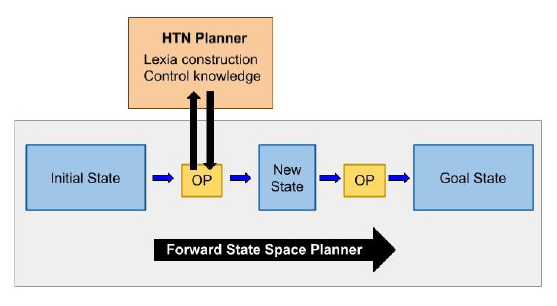
\includegraphics[totalheight=7cm]{1}}
    \caption{Planificador \textit{Story Assembler} y relación con fragmentos de textos. \cite{garbe2019storyassembler}}
    \label{fig:ptest1}
\end{figure}


\textit{Story Assembler} es un Sistema Deliberativo en donde se establecen los estados prioritarios que el sistema debe alcanzar. Funciona de manera  muy similar a un planificador \ac{HTN} pues crea eventos a partir de una librería de fragmentos de texto utilizando párrafos de textos más grandes. Cuando es ejecutado, \textit{Story Assembler} revisa las variables del estado inicial y las variables del estado deseado para posteriormente proceder a ensamblar fragmentos que lo acerquen cada vez más a su objetivo. Si el sistema ubica fragmentos de texto que lo acerquen de manera significativa, este procederá a juntarlos y tratarlos como un fragmento de texto único. Al final de una iteracción, el mejor fragmento esamblado representará el siguiente paso que el sistema dé para alcanzar su estado objetivo. 

\subsection{Let CONAN tell you a story} 

CONAN \cite{breault2018let} es un sistema de generación procedural de \textit{quest} aplicados en videojuegos (Muy similar a CARDINAL). Como casi todos los planificadores, funciona a partir de un estado inicial y de un conjunto que defina todas las posibles acciones a realizar en el mundo. CONAN es un sistema de simulación, es decir que a diferencia del modelo previo, acá no existen estados deseables que el sistema deba alcanzar. De hecho, podríamos definir a CONAN como un conjunto de pequeños agentes inteligentes de planeamiento. Cuando el sistema es puesto en marcha, cada \ac{NPC} dentro del juego revisará los objetivos que posee e implementará un plan que le será comunicado al jugador como un \textit{quest}. Por ejemplo, si un panadero \ac{NPC} se quedase sin material para seguir fabricando pan, entonce el planificador tras este identificará el nuevo problema de  conseguir Harina como un \textit{quest} para el jugador.

Para cada planificador en CONAN se requiere de los siguientes elementos:

\begin{itemize}
\item \textbf{Estado Inicial:} Es un estado estándar que representa el punto de partida para cada uno los \ac{NPC} y para el mundo en general. Definir un estado inicial en CONAN significa enfocarse en aspectos tales como: Localizaciones, Descripciones e Interconexiones. Además, cada pequeño agente en este sistema estará provisto de un conjunto de preferencias definidos en relación a un peso descrito en sus acciones. 

\item \textbf{Documento de Dominio:} Contiene todas las posibles acciones que puede realizar un personaje para poder alcanzar un objetivo. Más allá de estos, uno no podrá recurrir a acciones que lo fueron designadas.

\item \textbf{Generación de Objetivos: } Para cada planificador individual un objetivo es un estado que deber verdadero en el mundo solamente para el. En CONAN la definición de un objetivo puede realizarse de dos formas: Aleatoriamente y Aleatoriamente pero considerando las prioridades de cada planificador. 

\end{itemize}

\begin{figure}[tph!]
\centerline{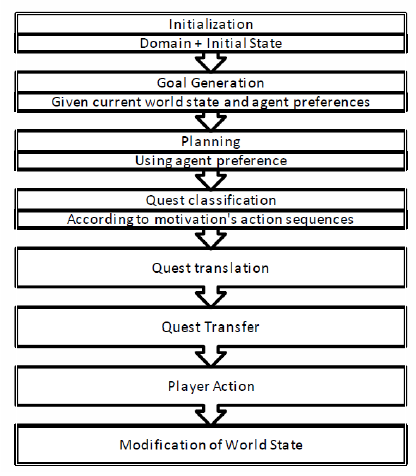
\includegraphics[totalheight=7cm]{2}}
    \caption{Desenvolvimiento del planificador \textit{CONAN}. \cite{breault2018let}}
    \label{fig:ptest1}
\end{figure}

\subsection{Story and Discourse}

Más que un sistema para la generación procedural de \textit{quests}, \textit{Story and Discourse} \cite{young2007story} es un modelo centrado en representar los dos aspectos básicos de la narrativa dentro de los mundos virtuales: Historia y Discurso. 

La historia se define como la serie de eventos por los que el personaje principal ha de pasar. Esta incluye además el planificador que se utilize (Para \textit{Story and Discourse} fue un planificador \ac{DPOCL}), algunos aspectos prácticos de la narratología como el suspenso, la originalidad o el interés y el porque se carece de modelos capaces de generar historias desde cero. 

Por otro lado, el discurso es el aspecto más práctico de la narratología. En este concepto se incluyen todas las formas que existen para transmitir una historia al jugador. Por ejemplo, si la historia de un videojuego señala el enfrentamiento entre antagonista y protagonista, el discurso de dicha historia sería cada fotograma que refleje dicho enfrentamiento. 
























%\section{Sección 1 del Capítulo II}

%Un capítulo puede contener n secciones. La referencia bibliográfica se hace de la siguiente manera: \cite{Mateos00}

%\subsection{Sub Sección}

%Una sección puede contener n sub secciones.\cite{Galante01}


%\section{Recomendaciones generales de escritura}
%Un trabajo de esta naturaleza debe tener en consideración varios aspectos generales:

%\begin{itemize}
%\item Ir de lo genérico a lo específico. Siempre hay qeu considerar que el lector podría ser alguien no muy familiar con el tema y la lectura debe serle atractiva.
%\item No poner frases muy largas. Si las frases son de mas de 2 líneas continuas es probable que la lectura sea dificultosa.
%\item Las figuras, ecuaciones, tablas deben ser citados y explicados {\bf antes} de que aparezcan en el documento.
%\item Encadenar las ideas. Ninguna frase debe estar suelta. Siempre que terminas un párrafo y hay otro a continuación,  el primero debe dejar abierta la idea que se explicará a continuación. Todo debe tener secuencia.
%\end{itemize}
